\section{Holographic Projections~\cite{Susskind1995} and Boundary Dynamics}

\subsection{The Hyper-Electron Internal Manifold as an Anti-de Sitter Bulk}

The central thesis of Excited-State Cosmology posits that the observable universe is the internal topological manifold of an excited hyper-electron, dynamically constrained by its asymptotic boundary—the 2D orbital shell. To formulate this mathematically, we map the interior bulk to an Anti-de Sitter ($AdS_{d+1}$) spacetime, where the negative cosmological constant arises from the vacuum energy of the hyper-electron's bounded excited state. \cite{Peebles1970, Harrison1970, Mukhanov1981}

We begin by establishing the metric of the $AdS_3$ bulk (a $2+1$ dimensional interior corresponding to our effective spatial manifold mapped into the lower-dimensional projection). In Poincaré coordinates, the metric is given by:
\begin{equation}
    ds^2 = \frac{L^2}{z^2} \left( -dt^2 + dx^2 + dz^2 \right),
\end{equation}
where $L$ is the AdS radius (fundamentally related to the Bohr-like radius of the hyper-electron state), and $z \in (0, \infty)$ is the holographic radial coordinate. The true boundary of the hyper-electron, the orbital shell, is located at the conformal boundary $z \to 0$.

The Riemann curvature tensor for this maximally symmetric space satisfies:
\begin{equation}
    R_{\mu\nu\rho\sigma} = -\frac{1}{L^2} \left( g_{\mu\rho} g_{\nu\sigma} - g_{\mu\sigma} g_{\nu\rho} \right),
\end{equation}
yielding a constant Ricci scalar $R = -\frac{d(d+1)}{L^2}$, which for $AdS_3$ evaluates to $-6/L^2$. This constant negative curvature represents the foundational tension of the excited hyper-electron maintaining its structural integrity against decay.

\subsection{The Holographic Dictionary: From Bulk Excitations to Orbital Shell}

According to the AdS/CFT correspondence~\cite{Maldacena1997}, quantum gravity in the $AdS_3$ bulk is dual to a Conformal Field Theory ($CFT_2$) on the 2D orbital shell. We define the generating functional equivalence:
\begin{equation}
    Z_{\text{bulk}}[\phi_0(x)] = \left\langle \exp\left( \int_{\partial \mathcal{M}} d^d x \, \phi_0(x) \mathcal{O}(x) \right) \right\rangle_{CFT},
\end{equation}
where $\phi_0(x)$ acts as a source for the boundary operator $\mathcal{O}(x)$.

To observe this mapping explicitly, consider a scalar field $\phi$ of mass $m$ propagating in the bulk, representing a localized energy fluctuation (a localized cosmic event) within the hyper-electron. The bulk action is:
\begin{equation}
    S = -\frac{1}{2\kappa^2} \int d^{d+1}x \sqrt{-g} \left( g^{\mu\nu} \partial_\mu \phi \partial_\nu \phi + m^2 \phi^2 \right).
\end{equation}
The corresponding Klein-Gordon equation of motion is $\left( \Box - m^2 \right) \phi = 0$. Expanding the d'Alembertian in Poincaré coordinates, we obtain:
\begin{equation}
    z^{d+1} \partial_z \left( z^{1-d} \partial_z \phi \right) + z^2 \eta^{ij} \partial_i \partial_j \phi - m^2 L^2 \phi = 0.
\end{equation}
We analyze the asymptotic behavior of $\phi$ near the orbital shell ($z \to 0$). Assuming a power-law solution $\phi \sim z^\Delta$, the equation reduces to the indicial constraint:
\begin{equation}
    \Delta(\Delta - d) - m^2 L^2 = 0.
\end{equation}
The roots of this characteristic equation are:
\begin{equation}
    \Delta_\pm = \frac{d}{2} \pm \sqrt{\frac{d^2}{4} + m^2 L^2}.
\end{equation}
Thus, the near-boundary expansion of the bulk field is:
\begin{equation}
    \phi(z, x) \sim z^{\Delta_-} \phi_0(x) + z^{\Delta_+} A(x), \quad (z \to 0).
\end{equation}
Here, $\phi_0(x)$ is the non-normalizable mode that sources the dual operator on the 2D orbital shell, and $A(x)$ is the normalizable mode associated with the expectation value $\langle \mathcal{O}(x) \rangle$. For stability (the Breitenlohner-Freedman bound), we require $m^2 L^2 \geq -d^2/4$. In the context of Excited-State Cosmology, this bound dictates the minimal stability criteria for macroscopic structures (galaxies, stellar clusters) surviving within the hyper-electron's interior without inducing catastrophic wave-function collapse.

\subsection{Ryu-Takayanagi~\cite{Ryu2006} Entropy and Orbital Entanglement}

To understand how the thermodynamics of the bulk universe reflect the quantum information on the orbital shell, we examine the entanglement entropy of a subregion. If we partition the 2D boundary $CFT$ into a spatial subregion $A$ and its complement $B$, the entanglement entropy is given by the von Neumann entropy $S_A = -\text{Tr}(\rho_A \ln \rho_A)$, where $\rho_A$ is the reduced density matrix.

The Ryu-Takayanagi (RT) formula elegantly geometrizes this entropy, stating that $S_A$ is proportional to the area of the minimal-area bulk surface $\gamma_A$ that is homologous to $A$ and anchored on its boundary $\partial A$:
\begin{equation}
    S_A = \frac{\text{Area}(\gamma_A)}{4G_N^{(d+1)}},
\end{equation}
where $G_N^{(d+1)}$ is the Newton constant in the bulk. 

We now derive this explicitly for the $AdS_3/CFT_2$ mapping of the hyper-electron. Let the boundary subregion $A$ be an interval of length $\ell$, denoted by $x \in [-\ell/2, \ell/2]$ at a constant time $t=0$. The bulk metric on this static slice simplifies to:
\begin{equation}
    ds^2 = \frac{L^2}{z^2} \left( dz^2 + dx^2 \right).
\end{equation}
We parameterize the curve $\gamma_A$ by $x(z)$. The length functional to be minimized is:
\begin{equation}
    \mathcal{L} = \int d\lambda \sqrt{g_{\mu\nu} \frac{dx^\mu}{d\lambda} \frac{dx^\nu}{d\lambda}} = \int_{-\ell/2}^{\ell/2} dx \frac{L}{z} \sqrt{1 + \left(\frac{dz}{dx}\right)^2}.
\end{equation}
Because the integrand does not depend explicitly on $x$, the associated Hamiltonian is a conserved quantity. By applying the Euler-Lagrange equations, we define the conserved "momentum":
\begin{equation}
    \frac{\partial \mathcal{L}}{\partial z'} z' - \mathcal{L} = \text{constant},
\end{equation}
where $z' = dz/dx$. Evaluating this gives:
\begin{equation}
    \frac{z' \frac{L}{z} \frac{z'}{\sqrt{1+(z')^2}} - \frac{L}{z} \sqrt{1+(z')^2}}{1} = -\frac{L}{z \sqrt{1+(z')^2}} = \text{constant} \equiv -\frac{L}{z_*}.
\end{equation}
Here, $z_*$ is the maximum depth the geodesic reaches into the hyper-electron bulk, where $z' = 0$. Solving the differential equation $\frac{dz}{dx} = \pm \frac{\sqrt{z_*^2 - z^2}}{z}$ yields the equation of a semicircle:
\begin{equation}
    x^2 + z^2 = z_*^2.
\end{equation}
Given the boundary conditions $z(\pm \ell/2) = 0$, we find that the turning point is exactly $z_* = \ell/2$.

To compute the length of this geodesic, we integrate along the semicircle. Due to the metric divergence at the conformal boundary $z \to 0$, we must introduce an ultraviolet (UV) cutoff $z = \epsilon$:
\begin{equation}
    \text{Length}(\gamma_A) = 2 \int_{\epsilon}^{\ell/2} dz \frac{dz}{dx} \frac{L}{z} \sqrt{1 + \left(\frac{dx}{dz}\right)^2}.
\end{equation}
Since $x^2 + z^2 = (\ell/2)^2$, we have $dx/dz = -z/x = -z/\sqrt{(\ell/2)^2 - z^2}$. Substituting this in:
\begin{equation}
    \text{Length}(\gamma_A) = 2L \int_{\epsilon}^{\ell/2} \frac{dz}{z \sqrt{1 - \left(\frac{2z}{\ell}\right)^2}}.
\end{equation}
Evaluating the integral gives:
\begin{equation}
    \text{Length}(\gamma_A) = 2L \ln \left( \frac{\ell}{\epsilon} \right).
\end{equation}
Substituting this back into the Ryu-Takayanagi formula gives the entanglement entropy of the region:
\begin{equation}
    S_A = \frac{2L \ln(\ell/\epsilon)}{4G_N^{(3)}} = \frac{L}{2G_N^{(3)}} \ln\left( \frac{\ell}{\epsilon} \right).
\end{equation}

Finally, to map this fully to the quantum mechanical properties of the orbital shell, we invoke the Brown-Henneaux relation, which dictates that any theory of gravity in $AdS_3$ must correspond to a $CFT_2$ with central charge:
\begin{equation}
    c = \frac{3L}{2G_N^{(3)}}.
\end{equation}
Substituting the central charge into our derived entropy expression yields:
\begin{equation}
    S_A = \frac{c}{3} \ln\left( \frac{\ell}{\epsilon} \right).
\end{equation}
This matches precisely the renowned Calabrese-Cardy formula derived via the replica trick in 2D Conformal Field Theory. 

In the paradigm of Excited-State Cosmology, this is a compelling demonstration: the entanglement thermodynamics measured on the 2D orbital shell of the hyper-electron are inextricably identical to the geometric gravitational degrees of freedom inside its 3D bulk volume. The expansion of our universe is thereby not a fluctuation of an isolated metric, but rather the quantum diffusion of entanglement across the hyper-electron's boundary state.


\begin{figure}[H]
\centering
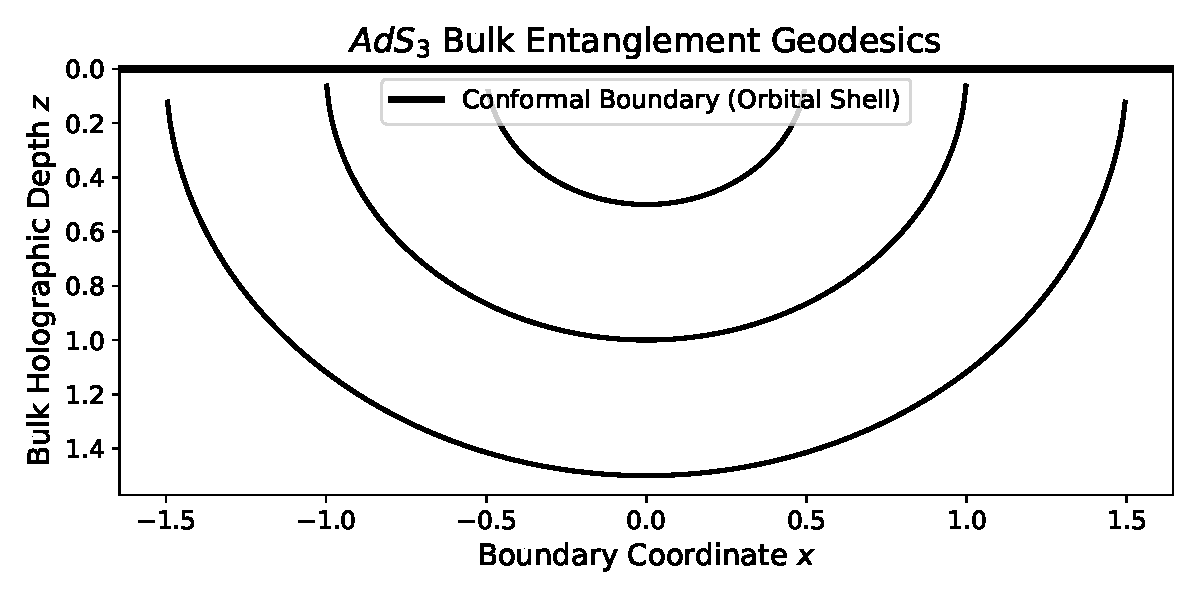
\includegraphics[width=0.85\textwidth]{fig_ch7.pdf}
\caption{Mathematical visualization of the principles derived in Section 7.}
\end{figure}
